%================================================================
%\chapter{Selection of Standard Probability Distributions}\label{sec:Appendix A}
\chapter{Standard Probability Distributions}\label{sec:Appendix A}
%================================================================


Summary statistics under the (noninformative) prior predictive distribution (draw 2000 samples, dropna -> left with 1703 samples, but here we only plot a subset of 425 samples)

\begin{figure}[H]
    \centering
    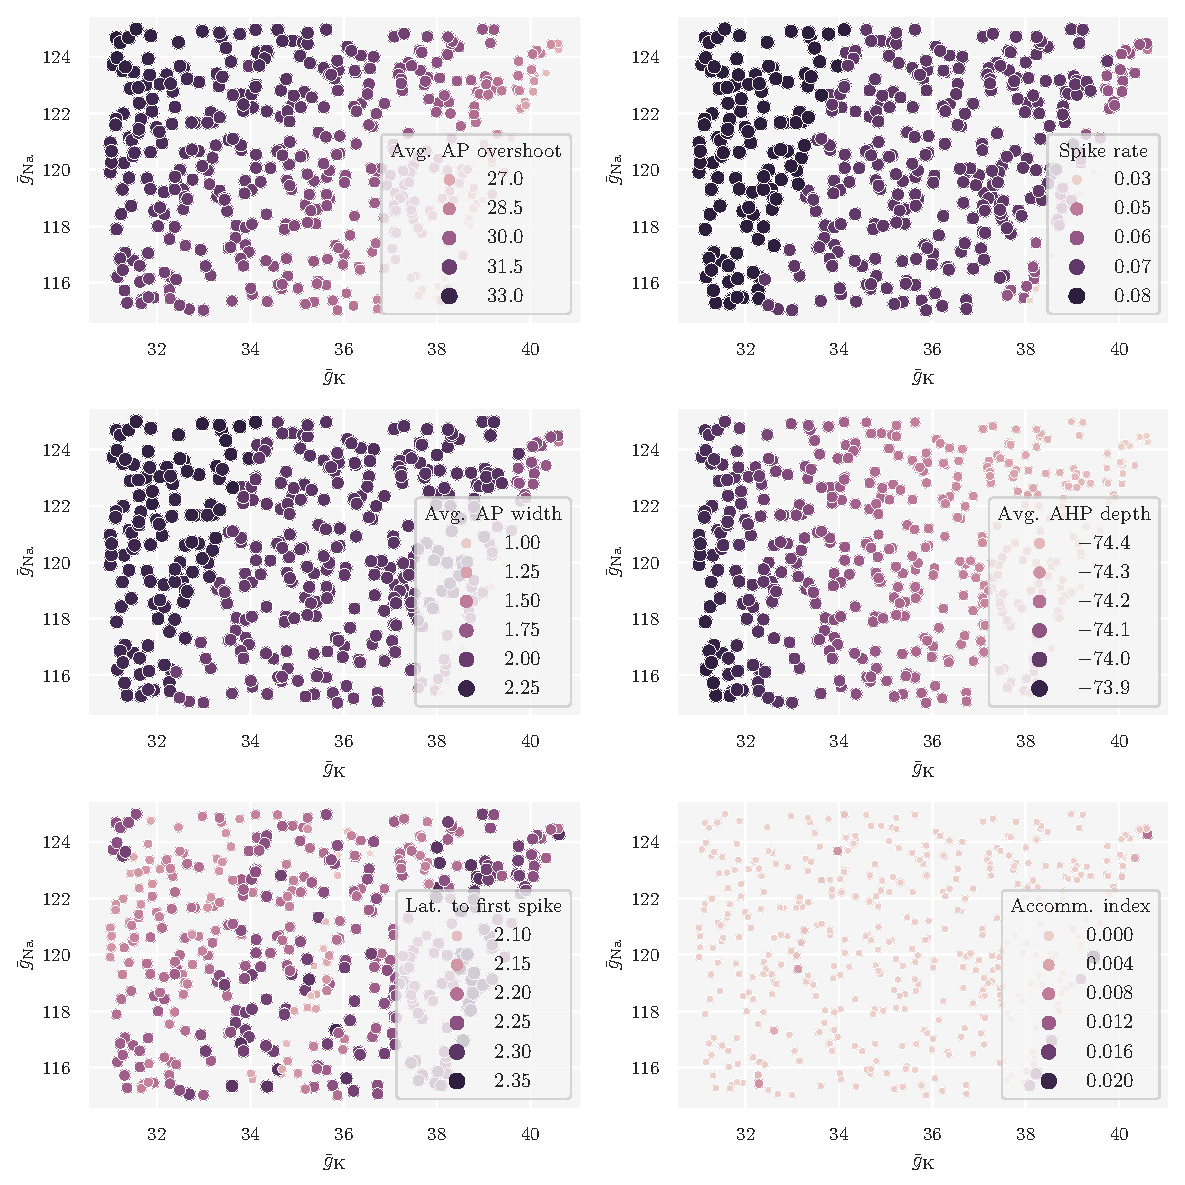
\includegraphics[scale=0.8]{hh_priorpred_sstats_uniform}
    \caption{caption}
    \label{fig:fig1}
\end{figure} 


Correlation (pearson) 

\begin{figure}[H]
    \centering
    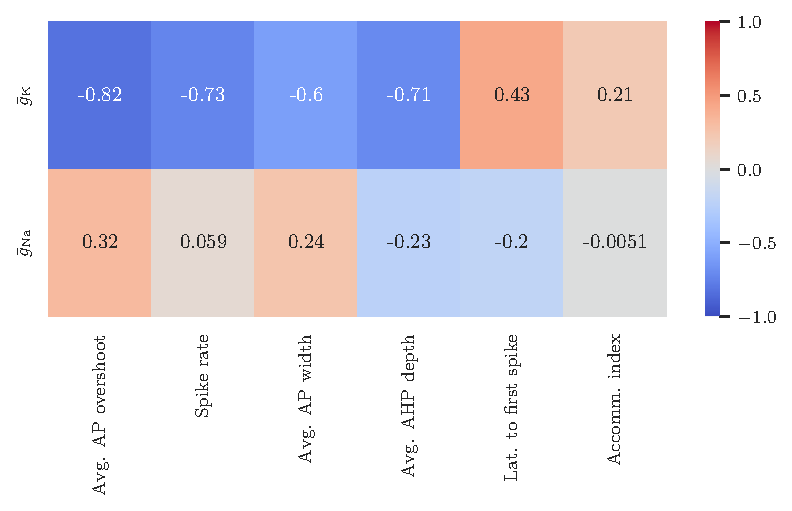
\includegraphics[scale=0.8]{hh_priorpred_corr_uniform}
    \caption{caption}
    \label{fig:fig1}
\end{figure} 

weights from corr coef

\begin{figure}[H]
    \centering
    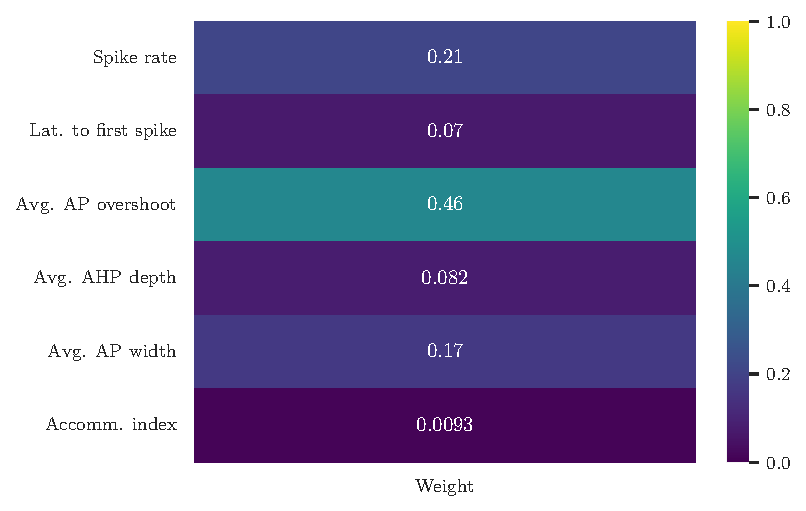
\includegraphics[scale=0.8]{hh_priorpred_weights_uniform}
    \caption{caption}
    \label{fig:fig1}
\end{figure} 

 
REJ-ABC hyperparam study 

num of pilot study simulations 

\begin{figure}[H]
    \centering
    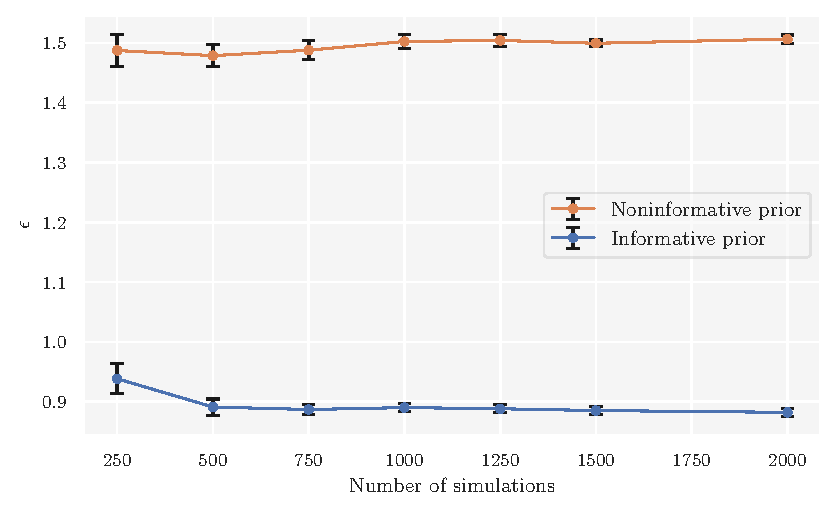
\includegraphics[scale=0.8]{pilot_eps_nsims}
    \caption{caption}
    \label{fig:fig1}
\end{figure} 

num of posterior draws

\begin{figure}[H]
    \centering
    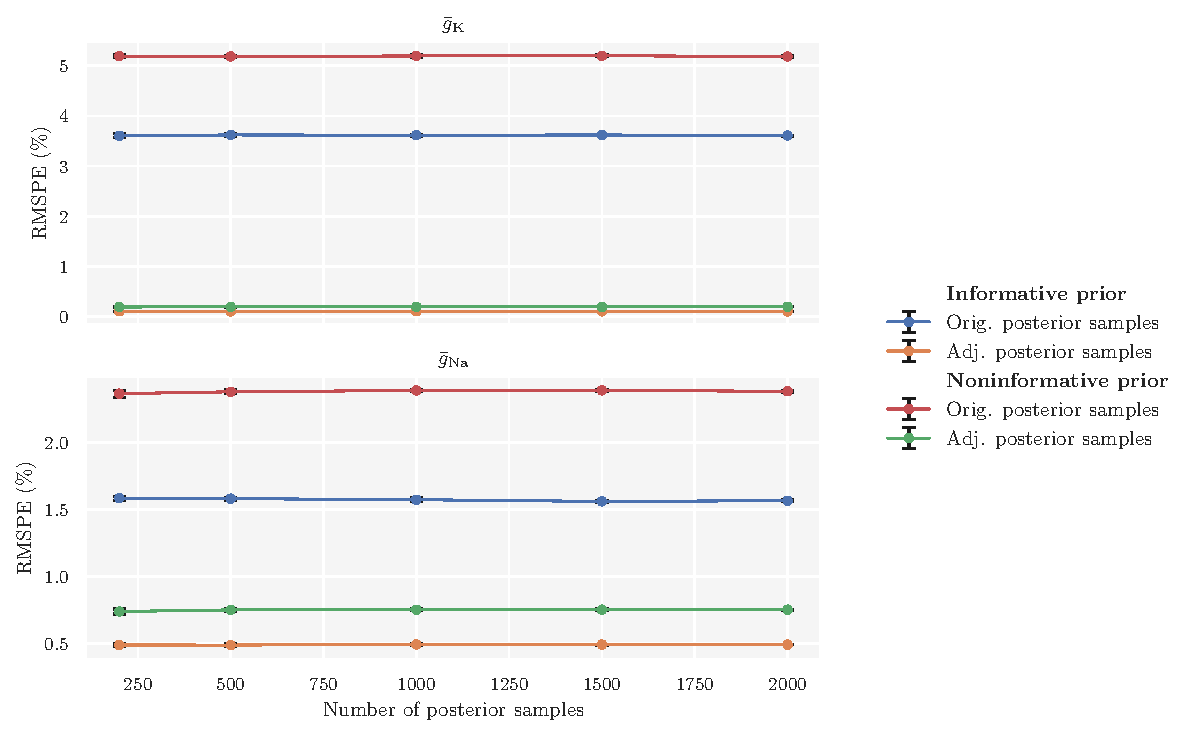
\includegraphics[scale=0.8]{RMSPE_vs_nsamples}
    \caption{caption}
    \label{fig:fig1}
\end{figure} 

----


A selection of standard probability 

Notation and formulas for several standard distributions appear in Appendix A 


about shape, location and scale parameters

template: 

distribution header

in table: 
distribution, parameters 
(name, symbol), (shape, location, scale)

pdf

about distribution


%================================================================
\section{Appendix.append(stuff)}
%================================================================

Appendix A

Standard distributions, see BDA appendix A

